%%%%%%%%%%%%%%%%%%%%%%%%%%%%%%%%%%%%%%%%%%%%%%%%%%%%%%%%%%%%
% 3.5 PROJECTIVE GEOMETRY
% The Composition of Advanced Mathematics
%%%%%%%%%%%%%%%%%%%%%%%%%%%%%%%%%%%%%%%%%%%%%%%%%%%%%%%%%%%%

\section{Projective Geometry}
\label{sec:projective-geometry}

\prerequisite{
Euclidean Geometry from \cref{sec:euclidean-geometry},
Analytic / Coordinate Geometry from
\cref{sec:analytic-coordinate-geometry},
Vector Geometry from \cref{sec:vector-geometry},
Affine Geometry from \cref{sec:affine-geometry},
and Linear Algebra from \cref{sec:linear-algebra}.
}

\learningobjectives{
By the end of this section, the reader should be able to:
\begin{itemize}
    \item explain the motivation for projective geometry;
    \item describe points at infinity and the projective completion of affine space;
    \item interpret projective points using homogeneous coordinates;
    \item work with the projective line and projective plane;
    \item convert between affine and projective coordinates;
    \item represent projective lines by homogeneous equations;
    \item compute intersections of projective lines;
    \item use cross products to calculate joins and intersections in
    \(\mathbb{P}^2\);
    \item explain the principle of projective duality;
    \item define and compute the cross-ratio;
    \item identify projective transformations using invertible matrices;
    \item distinguish affine and projective transformations;
    \item recognize projective invariants;
    \item describe conics in projective space;
    \item understand how affine conic classifications arise from projective
    geometry;
    \item connect projective geometry with perspective, computer vision,
    algebraic geometry, and geometry at infinity.
\end{itemize}
}

%%%%%%%%%%%%%%%%%%%%%%%%%%%%%%%%%%%%%%%%%%%%%%%%%%%%%%%%%%%%
\subsection{What Is Projective Geometry?}
\label{subsec:what-is-projective-geometry}
%%%%%%%%%%%%%%%%%%%%%%%%%%%%%%%%%%%%%%%%%%%%%%%%%%%%%%%%%%%%

Affine geometry preserves parallelism but treats parallel lines differently
from intersecting lines.

Projective geometry removes this distinction.

\begin{definitionbox}{Projective Geometry}
\emph{Projective geometry} studies geometric properties preserved under
projective transformations.

Its fundamental objects are points, lines, planes, incidence relations, and
projective invariants such as the cross-ratio.
\end{definitionbox}

A central principle is:

\[
\boxed{\text{In the projective plane, every two distinct lines intersect.}}
\]

Parallel affine lines acquire an intersection at a \emph{point at infinity}.

%%%%%%%%%%%%%%%%%%%%%%%%%%%%%%%%%%%%%%%%%%%%%%%%%%%%%%%%%%%%
\subsection{Why Introduce Points at Infinity?}
\label{subsec:why-points-at-infinity}
%%%%%%%%%%%%%%%%%%%%%%%%%%%%%%%%%%%%%%%%%%%%%%%%%%%%%%%%%%%%

Consider the affine lines

\[
y=0
\]

and

\[
y=1.
\]

They are parallel and therefore have no intersection in the affine plane.

Projective geometry enlarges the affine plane by adding ideal points.

The two lines are then said to meet at a point at infinity representing their
common direction.

\begin{centereddiagram}
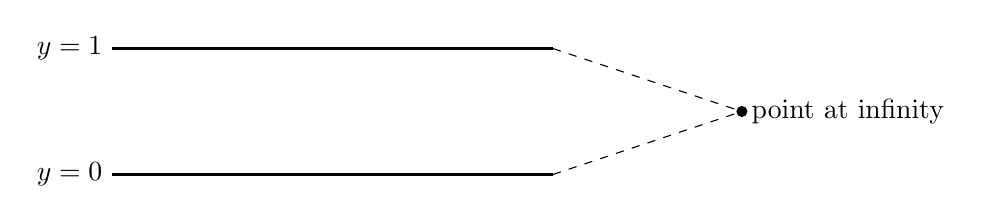
\begin{tikzpicture}[scale=0.8]
\draw[thick] (-4,-1)--(3,-1);
\draw[thick] (-4,1)--(3,1);

\draw[dashed] (3,-1)--(6,0);
\draw[dashed] (3,1)--(6,0);

\fill (6,0) circle (2.5pt);
\node[right] at (6,0) {point at infinity};

\node[left] at (-4,-1) {\(y=0\)};
\node[left] at (-4,1) {\(y=1\)};
\end{tikzpicture}
\end{centereddiagram}

The picture is schematic: the point at infinity is not an ordinary distant
Euclidean point.

It represents a direction.

%%%%%%%%%%%%%%%%%%%%%%%%%%%%%%%%%%%%%%%%%%%%%%%%%%%%%%%%%%%%
\subsection{Perspective as Motivation}
\label{subsec:projective-perspective-motivation}
%%%%%%%%%%%%%%%%%%%%%%%%%%%%%%%%%%%%%%%%%%%%%%%%%%%%%%%%%%%%

Projective geometry is closely connected with perspective drawing.

Railroad tracks are physically parallel, but in a perspective image they
appear to converge toward a vanishing point.

\begin{centereddiagram}
\begin{tikzpicture}[scale=0.85]
\coordinate (V) at (5,3);
\coordinate (A) at (0,0);
\coordinate (B) at (2,0);

\draw[thick] (A)--(V);
\draw[thick] (B)--(V);

\foreach \t in {0.12,0.25,0.4,0.58,0.78}{
    \coordinate (L) at ($(A)!\t!(V)$);
    \coordinate (R) at ($(B)!\t!(V)$);
    \draw (L)--(R);
}

\fill (V) circle (2.5pt);
\node[above] at (V) {vanishing point};
\end{tikzpicture}
\end{centereddiagram}

Vanishing points are practical manifestations of projective directions.

%%%%%%%%%%%%%%%%%%%%%%%%%%%%%%%%%%%%%%%%%%%%%%%%%%%%%%%%%%%%
\subsection{Homogeneous Coordinates}
\label{subsec:projective-homogeneous-coordinates}
%%%%%%%%%%%%%%%%%%%%%%%%%%%%%%%%%%%%%%%%%%%%%%%%%%%%%%%%%%%%

Affine Geometry introduced homogeneous coordinates as a convenient way to
represent affine transformations.

In projective geometry they become intrinsic.

\begin{definitionbox}{Homogeneous Coordinates}
A point of the real projective plane is represented by a nonzero triple

\[
(X,Y,Z)\in\R^3\setminus\{\mathbf{0}\},
\]

where proportional triples represent the same projective point:

\[
\boxed{
[X:Y:Z]=[\lambda X:\lambda Y:\lambda Z],
\qquad
\lambda\neq0.
}
\]

The notation \([X:Y:Z]\) is called \emph{homogeneous coordinates}.
\end{definitionbox}

Thus

\[
[1:2:3]
=
[2:4:6]
=
[-1:-2:-3].
\]

These are different vectors in \(\R^3\), but they represent the same
projective point.

%%%%%%%%%%%%%%%%%%%%%%%%%%%%%%%%%%%%%%%%%%%%%%%%%%%%%%%%%%%%
\subsection{Why Scaling Does Not Change a Projective Point}
\label{subsec:projective-scaling-equivalence}
%%%%%%%%%%%%%%%%%%%%%%%%%%%%%%%%%%%%%%%%%%%%%%%%%%%%%%%%%%%%

A projective point corresponds to a one-dimensional linear subspace through
the origin.

For example,

\[
[1:2:3]
\]

represents the line

\[
\{(t,2t,3t):t\in\R\}
\]

through the origin in \(\R^3\).

Multiplying the coordinates by a nonzero scalar merely chooses a different
nonzero vector on the same line.

Thus

\[
\boxed{
\text{projective point}
\longleftrightarrow
\text{one-dimensional linear subspace}.
}
\]

%%%%%%%%%%%%%%%%%%%%%%%%%%%%%%%%%%%%%%%%%%%%%%%%%%%%%%%%%%%%
\subsection{Projective Space}
\label{subsec:projective-space}
%%%%%%%%%%%%%%%%%%%%%%%%%%%%%%%%%%%%%%%%%%%%%%%%%%%%%%%%%%%%

\begin{definitionbox}{Real Projective Space}
The \(n\)-dimensional real projective space is

\[
\boxed{
\mathbb{P}^{n}(\R)
=
\left(\R^{n+1}\setminus\{\mathbf{0}\}\right)/\sim,
}
\]

where

\[
\mathbf{x}\sim\lambda\mathbf{x}
\]

for every nonzero scalar \(\lambda\).
\end{definitionbox}

The symbol

\[
\mathbb{P}^{n}
\]

is read ``projective \(n\)-space.''

Common examples are

\[
\mathbb{P}^{1},\qquad
\mathbb{P}^{2},\qquad
\mathbb{P}^{3}.
\]

They are called the projective line, projective plane, and projective
three-space.

%%%%%%%%%%%%%%%%%%%%%%%%%%%%%%%%%%%%%%%%%%%%%%%%%%%%%%%%%%%%
\subsection{The Projective Line}
\label{subsec:projective-line}
%%%%%%%%%%%%%%%%%%%%%%%%%%%%%%%%%%%%%%%%%%%%%%%%%%%%%%%%%%%%

A point of

\[
\mathbb{P}^{1}(\R)
\]

has coordinates

\[
[X:Z],
\]

not both zero.

When \(Z\neq0\), divide by \(Z\):

\[
[X:Z]
=
\left[\frac{X}{Z}:1\right].
\]

Thus the corresponding affine coordinate is

\[
x=\frac{X}{Z}.
\]

When

\[
Z=0,
\]

the only projective point is

\[
[1:0].
\]

Therefore

\[
\boxed{
\mathbb{P}^{1}(\R)
=
\R\cup\{\infty\}
}
\]

as a set, after choosing an affine coordinate chart.

The point

\[
[1:0]
\]

is the point at infinity of the real projective line.

%%%%%%%%%%%%%%%%%%%%%%%%%%%%%%%%%%%%%%%%%%%%%%%%%%%%%%%%%%%%
\subsection{The Projective Plane}
\label{subsec:projective-plane}
%%%%%%%%%%%%%%%%%%%%%%%%%%%%%%%%%%%%%%%%%%%%%%%%%%%%%%%%%%%%

Points of the real projective plane have coordinates

\[
[X:Y:Z].
\]

When

\[
Z\neq0,
\]

we may divide by \(Z\):

\[
[X:Y:Z]
=
\left[
\frac{X}{Z}:
\frac{Y}{Z}:
1
\right].
\]

This corresponds to the affine point

\[
\boxed{
(x,y)=
\left(
\frac{X}{Z},
\frac{Y}{Z}
\right).
}
\]

Thus ordinary affine points correspond to projective points with

\[
Z\neq0.
\]

%%%%%%%%%%%%%%%%%%%%%%%%%%%%%%%%%%%%%%%%%%%%%%%%%%%%%%%%%%%%
\subsection{The Line at Infinity}
\label{subsec:line-at-infinity}
%%%%%%%%%%%%%%%%%%%%%%%%%%%%%%%%%%%%%%%%%%%%%%%%%%%%%%%%%%%%

Points satisfying

\[
\boxed{Z=0}
\]

do not correspond to ordinary affine points.

They form the \emph{line at infinity}.

A typical point at infinity has the form

\[
[X:Y:0].
\]

Because homogeneous coordinates are defined only up to nonzero scaling,

\[
[X:Y:0]
=
[\lambda X:\lambda Y:0].
\]

Thus points at infinity encode directions in the affine plane.

%%%%%%%%%%%%%%%%%%%%%%%%%%%%%%%%%%%%%%%%%%%%%%%%%%%%%%%%%%%%
\subsection{Affine Directions as Projective Points}
\label{subsec:affine-directions-projective}
%%%%%%%%%%%%%%%%%%%%%%%%%%%%%%%%%%%%%%%%%%%%%%%%%%%%%%%%%%%%

An affine line with direction vector

\[
(a,b)
\]

has corresponding projective point at infinity

\[
\boxed{[a:b:0].}
\]

All parallel lines with direction \((a,b)\) pass through this same
projective point.

For example, all horizontal lines have direction

\[
(1,0),
\]

so their common point at infinity is

\[
\boxed{[1:0:0].}
\]

All vertical lines have direction

\[
(0,1),
\]

so their common point at infinity is

\[
\boxed{[0:1:0].}
\]

%%%%%%%%%%%%%%%%%%%%%%%%%%%%%%%%%%%%%%%%%%%%%%%%%%%%%%%%%%%%
\subsection{From Affine to Projective Coordinates}
\label{subsec:affine-to-projective}
%%%%%%%%%%%%%%%%%%%%%%%%%%%%%%%%%%%%%%%%%%%%%%%%%%%%%%%%%%%%

An affine point

\[
(x,y)
\]

is embedded into projective space by

\[
\boxed{
(x,y)\longmapsto[x:y:1].
}
\]

For example,

\[
(2,-3)
\longmapsto
[2:-3:1].
\]

Because homogeneous coordinates may be rescaled,

\[
[2:-3:1]
=
[4:-6:2].
\]

%%%%%%%%%%%%%%%%%%%%%%%%%%%%%%%%%%%%%%%%%%%%%%%%%%%%%%%%%%%%
\subsection{From Projective to Affine Coordinates}
\label{subsec:projective-to-affine}
%%%%%%%%%%%%%%%%%%%%%%%%%%%%%%%%%%%%%%%%%%%%%%%%%%%%%%%%%%%%

If

\[
[X:Y:Z]
\]

has \(Z\neq0\), then

\[
\boxed{
(x,y)=
\left(
\frac{X}{Z},
\frac{Y}{Z}
\right).
}
\]

For example,

\[
[6:9:3]
=
[2:3:1],
\]

so the corresponding affine point is

\[
\boxed{(2,3).}
\]

If \(Z=0\), no affine point is obtained in this coordinate chart.

%%%%%%%%%%%%%%%%%%%%%%%%%%%%%%%%%%%%%%%%%%%%%%%%%%%%%%%%%%%%
\subsection{Worked Example: Homogeneous Coordinates}
\label{subsec:worked-projective-homogeneous}
%%%%%%%%%%%%%%%%%%%%%%%%%%%%%%%%%%%%%%%%%%%%%%%%%%%%%%%%%%%%

\begin{workedexamplebox}{Converting Projective Coordinates}

Convert

\[
P=[8:-4:2]
\]

to affine coordinates.

\begin{tabularx}{\textwidth}{@{}>{\raggedright\arraybackslash}p{0.43\textwidth}X@{}}
Check the final coordinate. &
\(Z=2\neq0\)\\
Divide by \(Z\). &
\([8:-4:2]=[4:-2:1]\)\\
Read the affine coordinates. &
\((x,y)=(4,-2)\)
\end{tabularx}

\begin{answerbox}
\[
\boxed{P=(4,-2)}
\]
\end{answerbox}
\end{workedexamplebox}

%%%%%%%%%%%%%%%%%%%%%%%%%%%%%%%%%%%%%%%%%%%%%%%%%%%%%%%%%%%%
\subsection{Projective Lines}
\label{subsec:projective-lines}
%%%%%%%%%%%%%%%%%%%%%%%%%%%%%%%%%%%%%%%%%%%%%%%%%%%%%%%%%%%%

A projective line in \(\mathbb{P}^{2}\) is represented by a homogeneous
linear equation

\[
\boxed{
aX+bY+cZ=0,
}
\]

where

\[
(a,b,c)\neq(0,0,0).
\]

Multiplying all coefficients by a nonzero scalar does not change the line.

Thus

\[
aX+bY+cZ=0
\]

and

\[
\lambda aX+\lambda bY+\lambda cZ=0
\]

represent the same projective line.

%%%%%%%%%%%%%%%%%%%%%%%%%%%%%%%%%%%%%%%%%%%%%%%%%%%%%%%%%%%%
\subsection{Affine Lines Inside the Projective Plane}
\label{subsec:affine-lines-projective-plane}
%%%%%%%%%%%%%%%%%%%%%%%%%%%%%%%%%%%%%%%%%%%%%%%%%%%%%%%%%%%%

An affine line

\[
ax+by+c=0
\]

becomes

\[
\boxed{
aX+bY+cZ=0
}
\]

after homogenization.

Indeed, substituting

\[
x=\frac{X}{Z},
\qquad
y=\frac{Y}{Z}
\]

and multiplying by \(Z\) gives the homogeneous equation.

%%%%%%%%%%%%%%%%%%%%%%%%%%%%%%%%%%%%%%%%%%%%%%%%%%%%%%%%%%%%
\subsection{Homogenization}
\label{subsec:projective-homogenization}
%%%%%%%%%%%%%%%%%%%%%%%%%%%%%%%%%%%%%%%%%%%%%%%%%%%%%%%%%%%%

The process of converting an affine polynomial equation into a homogeneous
projective equation is called \emph{homogenization}.

For example,

\[
x^2+y^2=1
\]

becomes

\[
\boxed{
X^2+Y^2=Z^2.
}
\]

Similarly,

\[
y=x^2
\]

becomes

\[
\boxed{
YZ=X^2.
}
\]

Every term in the homogenized equation has the same total degree.

%%%%%%%%%%%%%%%%%%%%%%%%%%%%%%%%%%%%%%%%%%%%%%%%%%%%%%%%%%%%
\subsection{Dehomogenization}
\label{subsec:projective-dehomogenization}
%%%%%%%%%%%%%%%%%%%%%%%%%%%%%%%%%%%%%%%%%%%%%%%%%%%%%%%%%%%%

To recover an affine equation in the chart \(Z\neq0\), set

\[
Z=1.
\]

For example,

\[
X^2+Y^2-Z^2=0
\]

becomes

\[
x^2+y^2-1=0.
\]

This process is called \emph{dehomogenization}.

%%%%%%%%%%%%%%%%%%%%%%%%%%%%%%%%%%%%%%%%%%%%%%%%%%%%%%%%%%%%
\subsection{Incidence}
\label{subsec:projective-incidence}
%%%%%%%%%%%%%%%%%%%%%%%%%%%%%%%%%%%%%%%%%%%%%%%%%%%%%%%%%%%%

A point

\[
P=[X:Y:Z]
\]

lies on the line

\[
\ell=[a:b:c]
\]

when

\[
\boxed{
aX+bY+cZ=0.
}
\]

The word \emph{incidence} refers to relationships such as:

\begin{itemize}
    \item a point lying on a line;
    \item a line passing through a point;
    \item several lines meeting at one point.
\end{itemize}

Incidence is one of the central structures preserved by projective
transformations.

%%%%%%%%%%%%%%%%%%%%%%%%%%%%%%%%%%%%%%%%%%%%%%%%%%%%%%%%%%%%
\subsection{Lines as Homogeneous Coordinates}
\label{subsec:line-homogeneous-coordinates}
%%%%%%%%%%%%%%%%%%%%%%%%%%%%%%%%%%%%%%%%%%%%%%%%%%%%%%%%%%%%

A projective line

\[
aX+bY+cZ=0
\]

may itself be represented by the homogeneous triple

\[
\boxed{\ell=[a:b:c].}
\]

This creates a remarkable symmetry:

\[
\text{point }P=[X:Y:Z],
\]

while

\[
\text{line }\ell=[a:b:c].
\]

Incidence becomes

\[
\boxed{\ell^{T}P=0.}
\]

This symmetry is the basis of projective duality.

%%%%%%%%%%%%%%%%%%%%%%%%%%%%%%%%%%%%%%%%%%%%%%%%%%%%%%%%%%%%
\subsection{The Line Through Two Points}
\label{subsec:projective-line-through-points}
%%%%%%%%%%%%%%%%%%%%%%%%%%%%%%%%%%%%%%%%%%%%%%%%%%%%%%%%%%%%

Let

\[
P=[X_1:Y_1:Z_1]
\]

and

\[
Q=[X_2:Y_2:Z_2].
\]

The line through them can be computed using the cross product:

\[
\boxed{
\ell=P\times Q.
}
\]

Writing the homogeneous coordinate vectors as columns,

\[
P=
\begin{pmatrix}
X_1\\Y_1\\Z_1
\end{pmatrix},
\qquad
Q=
\begin{pmatrix}
X_2\\Y_2\\Z_2
\end{pmatrix},
\]

the vector

\[
P\times Q
\]

gives the coefficients of the line equation.

%%%%%%%%%%%%%%%%%%%%%%%%%%%%%%%%%%%%%%%%%%%%%%%%%%%%%%%%%%%%
\subsection{Worked Example: Line Through Two Points}
\label{subsec:worked-projective-line-two-points}
%%%%%%%%%%%%%%%%%%%%%%%%%%%%%%%%%%%%%%%%%%%%%%%%%%%%%%%%%%%%

\begin{workedexamplebox}{Finding a Projective Line}

Find the projective line through

\[
P=[1:0:1],
\qquad
Q=[0:1:1].
\]

Compute

\[
P\times Q
=
\begin{pmatrix}
1\\0\\1
\end{pmatrix}
\times
\begin{pmatrix}
0\\1\\1
\end{pmatrix}.
\]

\begin{tabularx}{\textwidth}{@{}>{\raggedright\arraybackslash}p{0.43\textwidth}X@{}}
Compute the cross product. &
\(P\times Q=(-1,-1,1)\)\\
Use the result as line coefficients. &
\(-X-Y+Z=0\)\\
Rescale if desired. &
\(X+Y-Z=0\)
\end{tabularx}

\begin{answerbox}
\[
\boxed{X+Y-Z=0}
\]
\end{answerbox}
\end{workedexamplebox}

%%%%%%%%%%%%%%%%%%%%%%%%%%%%%%%%%%%%%%%%%%%%%%%%%%%%%%%%%%%%
\subsection{Intersection of Two Lines}
\label{subsec:intersection-projective-lines}
%%%%%%%%%%%%%%%%%%%%%%%%%%%%%%%%%%%%%%%%%%%%%%%%%%%%%%%%%%%%

The dual operation is equally simple.

If

\[
\ell_1=[a_1:b_1:c_1]
\]

and

\[
\ell_2=[a_2:b_2:c_2],
\]

then their intersection point is

\[
\boxed{
P=\ell_1\times\ell_2.
}
\]

This formula works even when the corresponding affine lines are parallel.

%%%%%%%%%%%%%%%%%%%%%%%%%%%%%%%%%%%%%%%%%%%%%%%%%%%%%%%%%%%%
\subsection{Worked Example: Parallel Lines Meet at Infinity}
\label{subsec:worked-parallel-lines-infinity}
%%%%%%%%%%%%%%%%%%%%%%%%%%%%%%%%%%%%%%%%%%%%%%%%%%%%%%%%%%%%

\begin{workedexamplebox}{Finding the Intersection of Parallel Lines}

Consider

\[
y=1
\]

and

\[
y=3.
\]

Their projective equations are

\[
Y-Z=0
\]

and

\[
Y-3Z=0.
\]

Thus

\[
\ell_1=[0:1:-1],
\qquad
\ell_2=[0:1:-3].
\]

Compute

\[
\ell_1\times\ell_2.
\]

\begin{tabularx}{\textwidth}{@{}>{\raggedright\arraybackslash}p{0.43\textwidth}X@{}}
Compute the cross product. &
\(\ell_1\times\ell_2=(-2,0,0)\)\\
Rescale the homogeneous coordinates. &
\([-2:0:0]=[1:0:0]\)\\
Interpret \(Z=0\). &
The intersection is a point at infinity.
\end{tabularx}

\begin{answerbox}
\[
\boxed{[1:0:0]}
\]

The horizontal lines meet at the projective point representing the
horizontal direction.
\end{answerbox}
\end{workedexamplebox}

%%%%%%%%%%%%%%%%%%%%%%%%%%%%%%%%%%%%%%%%%%%%%%%%%%%%%%%%%%%%
\subsection{Every Two Lines Intersect}
\label{subsec:every-two-projective-lines-intersect}
%%%%%%%%%%%%%%%%%%%%%%%%%%%%%%%%%%%%%%%%%%%%%%%%%%%%%%%%%%%%

Two distinct projective lines correspond to two linearly independent
coefficient vectors

\[
\ell_1,\ell_2\in\R^3.
\]

Their cross product is nonzero:

\[
\ell_1\times\ell_2\neq0.
\]

Therefore it represents a projective point.

Hence:

\begin{theorem}[Intersection Property of the Projective Plane]
Every two distinct projective lines in \(\mathbb{P}^{2}(\R)\) intersect in
exactly one projective point.
\end{theorem}

This removes the exceptional parallel case found in affine geometry.

%%%%%%%%%%%%%%%%%%%%%%%%%%%%%%%%%%%%%%%%%%%%%%%%%%%%%%%%%%%%
\subsection{Every Two Points Determine a Line}
\label{subsec:two-points-projective-line}
%%%%%%%%%%%%%%%%%%%%%%%%%%%%%%%%%%%%%%%%%%%%%%%%%%%%%%%%%%%%

Similarly:

\begin{theorem}[Join Property of the Projective Plane]
Every two distinct points in \(\mathbb{P}^{2}(\R)\) lie on exactly one
projective line.
\end{theorem}

The line is

\[
\boxed{\ell=P\times Q.}
\]

The operation of constructing the line through two points is often called
their \emph{join}.

The intersection of two lines is often called their \emph{meet}.

%%%%%%%%%%%%%%%%%%%%%%%%%%%%%%%%%%%%%%%%%%%%%%%%%%%%%%%%%%%%
\subsection{Join and Meet}
\label{subsec:projective-join-meet}
%%%%%%%%%%%%%%%%%%%%%%%%%%%%%%%%%%%%%%%%%%%%%%%%%%%%%%%%%%%%

In the projective plane:

\[
\boxed{
\text{join of points: }
P\vee Q=P\times Q
}
\]

and

\[
\boxed{
\text{meet of lines: }
\ell_1\wedge\ell_2=\ell_1\times\ell_2.
}
\]

The symbols

\[
\vee
\qquad\text{and}\qquad
\wedge
\]

are read ``join'' and ``meet'' in this context.

These operations emphasize the dual roles of points and lines.

%%%%%%%%%%%%%%%%%%%%%%%%%%%%%%%%%%%%%%%%%%%%%%%%%%%%%%%%%%%%
\subsection{Projective Duality}
\label{subsec:projective-duality}
%%%%%%%%%%%%%%%%%%%%%%%%%%%%%%%%%%%%%%%%%%%%%%%%%%%%%%%%%%%%

Projective geometry exhibits a deep symmetry between points and lines.

A statement such as

\[
\text{two points determine a unique line}
\]

has the dual statement

\[
\text{two lines determine a unique point}.
\]

\begin{importantbox}
The \emph{principle of projective duality} states, roughly, that many valid
theorems in the projective plane remain valid after interchanging the roles
of points and lines, together with the corresponding incidence relations.
\end{importantbox}

This is not merely a linguistic coincidence.

It reflects the linear-algebraic duality between one-dimensional and
codimension-one subspaces.

%%%%%%%%%%%%%%%%%%%%%%%%%%%%%%%%%%%%%%%%%%%%%%%%%%%%%%%%%%%%
\subsection{Collinearity}
\label{subsec:projective-collinearity}
%%%%%%%%%%%%%%%%%%%%%%%%%%%%%%%%%%%%%%%%%%%%%%%%%%%%%%%%%%%%

Three projective points

\[
P,\qquad Q,\qquad R
\]

are collinear precisely when their homogeneous coordinate vectors are
linearly dependent.

Equivalently,

\[
\boxed{
\det
\begin{pmatrix}
X_P&Y_P&Z_P\\
X_Q&Y_Q&Z_Q\\
X_R&Y_R&Z_R
\end{pmatrix}
=0.
}
\]

Thus projective incidence questions can often be reduced to determinant
computations.

%%%%%%%%%%%%%%%%%%%%%%%%%%%%%%%%%%%%%%%%%%%%%%%%%%%%%%%%%%%%
\subsection{Concurrency}
\label{subsec:projective-concurrency}
%%%%%%%%%%%%%%%%%%%%%%%%%%%%%%%%%%%%%%%%%%%%%%%%%%%%%%%%%%%%

Three projective lines

\[
\ell_1,\qquad\ell_2,\qquad\ell_3
\]

are concurrent if they pass through one common point.

If

\[
\ell_i=[a_i:b_i:c_i],
\]

then concurrency occurs precisely when

\[
\boxed{
\det
\begin{pmatrix}
a_1&b_1&c_1\\
a_2&b_2&c_2\\
a_3&b_3&c_3
\end{pmatrix}
=0.
}
\]

This is the dual form of the collinearity criterion.

%%%%%%%%%%%%%%%%%%%%%%%%%%%%%%%%%%%%%%%%%%%%%%%%%%%%%%%%%%%%
\subsection{Projective Transformations}
\label{subsec:projective-transformations}
%%%%%%%%%%%%%%%%%%%%%%%%%%%%%%%%%%%%%%%%%%%%%%%%%%%%%%%%%%%%

Affine transformations use matrices together with translations.

Projective transformations arise naturally from invertible linear maps on
homogeneous coordinates.

\begin{definitionbox}{Projective Transformation}
Let

\[
A\in GL(n+1,\R).
\]

The transformation

\[
\boxed{
[\mathbf{x}]
\longmapsto
[A\mathbf{x}]
}
\]

defines a \emph{projective transformation} of
\(\mathbb{P}^{n}(\R)\).
\end{definitionbox}

Because homogeneous coordinates are defined up to nonzero scalar
multiplication, scalar multiples of \(A\) define the same projective
transformation.

%%%%%%%%%%%%%%%%%%%%%%%%%%%%%%%%%%%%%%%%%%%%%%%%%%%%%%%%%%%%
\subsection{The Projective Linear Group}
\label{subsec:projective-linear-group}
%%%%%%%%%%%%%%%%%%%%%%%%%%%%%%%%%%%%%%%%%%%%%%%%%%%%%%%%%%%%

The group of projective linear transformations is denoted

\[
\boxed{
PGL(n+1,\R).
}
\]

The notation is read ``projective general linear group.''

Conceptually,

\[
PGL(n+1,\R)
=
GL(n+1,\R)
/\{\lambda I:\lambda\neq0\}.
\]

Matrices differing by a nonzero scalar represent the same projective
transformation.

%%%%%%%%%%%%%%%%%%%%%%%%%%%%%%%%%%%%%%%%%%%%%%%%%%%%%%%%%%%%
\subsection{Affine Transformations as Projective Transformations}
\label{subsec:affine-as-projective}
%%%%%%%%%%%%%%%%%%%%%%%%%%%%%%%%%%%%%%%%%%%%%%%%%%%%%%%%%%%%

An affine transformation

\[
\mathbf{x}\mapsto A\mathbf{x}+\mathbf{b}
\]

has homogeneous matrix

\[
\begin{pmatrix}
A&\mathbf{b}\\
\mathbf{0}^{T}&1
\end{pmatrix}.
\]

Therefore every invertible affine transformation extends to a projective
transformation.

However, projective transformations are more general.

A general projective transformation need not preserve the affine line at
infinity.

Consequently, it need not preserve parallelism.

%%%%%%%%%%%%%%%%%%%%%%%%%%%%%%%%%%%%%%%%%%%%%%%%%%%%%%%%%%%%
\subsection{Projective Transformation in Affine Coordinates}
\label{subsec:projective-transformation-affine-coordinates}
%%%%%%%%%%%%%%%%%%%%%%%%%%%%%%%%%%%%%%%%%%%%%%%%%%%%%%%%%%%%

Consider a projective transformation of \(\mathbb{P}^{2}\) represented by

\[
H=
\begin{pmatrix}
a&b&c\\
d&e&f\\
g&h&i
\end{pmatrix}.
\]

An affine point is represented by

\[
[x:y:1].
\]

After multiplication,

\[
H
\begin{pmatrix}
x\\y\\1
\end{pmatrix}
=
\begin{pmatrix}
ax+by+c\\
dx+ey+f\\
gx+hy+i
\end{pmatrix}.
\]

If the final coordinate is nonzero, the transformed affine point is

\[
\boxed{
x'
=
\frac{ax+by+c}{gx+hy+i},
\qquad
y'
=
\frac{dx+ey+f}{gx+hy+i}.
}
\]

Unlike affine transformations, the coordinates may involve division by
linear expressions.

%%%%%%%%%%%%%%%%%%%%%%%%%%%%%%%%%%%%%%%%%%%%%%%%%%%%%%%%%%%%
\subsection{Homographies}
\label{subsec:homographies}
%%%%%%%%%%%%%%%%%%%%%%%%%%%%%%%%%%%%%%%%%%%%%%%%%%%%%%%%%%%%

Projective transformations are also called \emph{homographies} or
\emph{projectivities} in many contexts.

On the projective line, a projective transformation has the form

\[
\boxed{
x\longmapsto\frac{ax+b}{cx+d},
}
\]

where

\[
ad-bc\neq0.
\]

These are also known as fractional linear or Möbius transformations.

Their complex-analytic theory is developed more fully in Complex Analysis.

%%%%%%%%%%%%%%%%%%%%%%%%%%%%%%%%%%%%%%%%%%%%%%%%%%%%%%%%%%%%
\subsection{Worked Example: Projective Transformation}
\label{subsec:worked-projective-transformation}
%%%%%%%%%%%%%%%%%%%%%%%%%%%%%%%%%%%%%%%%%%%%%%%%%%%%%%%%%%%%

\begin{workedexamplebox}{Applying a Projective Transformation}

Let

\[
H=
\begin{pmatrix}
1&0&2\\
0&1&1\\
1&0&1
\end{pmatrix}
\]

and let

\[
P=(1,2).
\]

Write \(P\) homogeneously:

\[
P=[1:2:1].
\]

Then

\[
H
\begin{pmatrix}
1\\2\\1
\end{pmatrix}
=
\begin{pmatrix}
3\\3\\2
\end{pmatrix}.
\]

Thus

\[
P'=[3:3:2].
\]

Dehomogenizing gives

\[
P'=
\left(
\frac32,
\frac32
\right).
\]

\begin{answerbox}
\[
\boxed{
T(1,2)=
\left(\frac32,\frac32\right)
}
\]
\end{answerbox}
\end{workedexamplebox}

%%%%%%%%%%%%%%%%%%%%%%%%%%%%%%%%%%%%%%%%%%%%%%%%%%%%%%%%%%%%
\subsection{Projective Invariants}
\label{subsec:projective-invariants}
%%%%%%%%%%%%%%%%%%%%%%%%%%%%%%%%%%%%%%%%%%%%%%%%%%%%%%%%%%%%

Projective transformations preserve less structure than affine
transformations.

They preserve:

\begin{itemize}
    \item points;
    \item lines;
    \item incidence;
    \item collinearity;
    \item concurrency;
    \item projective dimension;
    \item cross-ratios of four collinear points;
    \item projective equivalence of nondegenerate conics.
\end{itemize}

They do not generally preserve:

\begin{itemize}
    \item lengths;
    \item angles;
    \item perpendicularity;
    \item midpoints;
    \item ordinary ratios of lengths;
    \item parallelism;
    \item affine area.
\end{itemize}

%%%%%%%%%%%%%%%%%%%%%%%%%%%%%%%%%%%%%%%%%%%%%%%%%%%%%%%%%%%%
\subsection{The Cross-Ratio}
\label{subsec:cross-ratio}
%%%%%%%%%%%%%%%%%%%%%%%%%%%%%%%%%%%%%%%%%%%%%%%%%%%%%%%%%%%%

Ordinary distance ratios are not preserved by general projective
transformations.

A special combination of ratios is preserved.

\begin{definitionbox}{Cross-Ratio}
For four distinct collinear affine points with coordinates

\[
a,b,c,d,
\]

their \emph{cross-ratio} is

\[
\boxed{
(a,b;c,d)
=
\frac{(c-a)(d-b)}
     {(c-b)(d-a)}.
}
\]
\end{definitionbox}

The notation

\[
(a,b;c,d)
\]

is read ``the cross-ratio of \(a,b;c,d\).''

Different ordering conventions occur in the literature, so the chosen
formula should always be stated explicitly.

%%%%%%%%%%%%%%%%%%%%%%%%%%%%%%%%%%%%%%%%%%%%%%%%%%%%%%%%%%%%
\subsection{Worked Example: Cross-Ratio}
\label{subsec:worked-cross-ratio}
%%%%%%%%%%%%%%%%%%%%%%%%%%%%%%%%%%%%%%%%%%%%%%%%%%%%%%%%%%%%

\begin{workedexamplebox}{Computing a Cross-Ratio}

Compute

\[
(0,1;2,3).
\]

Using

\[
(a,b;c,d)
=
\frac{(c-a)(d-b)}
     {(c-b)(d-a)},
\]

we obtain

\[
(0,1;2,3)
=
\frac{(2-0)(3-1)}
     {(2-1)(3-0)}.
\]

Therefore

\[
=
\frac{2\cdot2}{1\cdot3}
=
\frac43.
\]

\begin{answerbox}
\[
\boxed{(0,1;2,3)=\frac43}
\]
\end{answerbox}
\end{workedexamplebox}

%%%%%%%%%%%%%%%%%%%%%%%%%%%%%%%%%%%%%%%%%%%%%%%%%%%%%%%%%%%%
\subsection{Cross-Ratio Invariance}
\label{subsec:cross-ratio-invariance}
%%%%%%%%%%%%%%%%%%%%%%%%%%%%%%%%%%%%%%%%%%%%%%%%%%%%%%%%%%%%

\begin{theorem}[Cross-Ratio Invariance]
Let

\[
T(x)=\frac{\alpha x+\beta}{\gamma x+\delta}
\]

be a projective transformation of the projective line.

Then, whenever the expressions are defined,

\[
\boxed{
(T(a),T(b);T(c),T(d))
=
(a,b;c,d).
}
\]
\end{theorem}

Thus the cross-ratio replaces ordinary length ratios as a fundamental
one-dimensional projective invariant.

%%%%%%%%%%%%%%%%%%%%%%%%%%%%%%%%%%%%%%%%%%%%%%%%%%%%%%%%%%%%
\subsection{Harmonic Division}
\label{subsec:harmonic-division}
%%%%%%%%%%%%%%%%%%%%%%%%%%%%%%%%%%%%%%%%%%%%%%%%%%%%%%%%%%%%

A particularly important configuration occurs when the cross-ratio is

\[
-1.
\]

\begin{definitionbox}{Harmonic Range}
Four collinear points form a \emph{harmonic range} when, under the convention
used in this section,

\[
\boxed{
(A,B;C,D)=-1.
}
\]
\end{definitionbox}

Harmonic configurations are preserved by projective transformations and play
an important role in classical projective geometry.

%%%%%%%%%%%%%%%%%%%%%%%%%%%%%%%%%%%%%%%%%%%%%%%%%%%%%%%%%%%%
\subsection{Projective Frames}
\label{subsec:projective-frames}
%%%%%%%%%%%%%%%%%%%%%%%%%%%%%%%%%%%%%%%%%%%%%%%%%%%%%%%%%%%%

Just as affine frames provide coordinate systems in affine geometry,
projective frames provide coordinate systems in projective geometry.

In \(\mathbb{P}^{n}\), a projective frame consists of \(n+2\) suitably
positioned points.

In the projective plane, four points in general position determine a
projective coordinate frame.

This is one reason projective transformations have more freedom than affine
transformations.

%%%%%%%%%%%%%%%%%%%%%%%%%%%%%%%%%%%%%%%%%%%%%%%%%%%%%%%%%%%%
\subsection{Four Points Determine a Projectivity}
\label{subsec:four-points-projectivity}
%%%%%%%%%%%%%%%%%%%%%%%%%%%%%%%%%%%%%%%%%%%%%%%%%%%%%%%%%%%%

On the projective line, a projective transformation is uniquely determined
by the images of three distinct points.

In the projective plane, a projective transformation is determined by the
images of a projective frame: four points in general position.

The phrase \emph{general position} here means that no three of the four
points are collinear.

%%%%%%%%%%%%%%%%%%%%%%%%%%%%%%%%%%%%%%%%%%%%%%%%%%%%%%%%%%%%
\subsection{The Fundamental Theorem of Projective Geometry}
\label{subsec:fundamental-theorem-projective-geometry}
%%%%%%%%%%%%%%%%%%%%%%%%%%%%%%%%%%%%%%%%%%%%%%%%%%%%%%%%%%%%

A central structural result explains why linear algebra appears throughout
projective geometry.

\begin{theorem}[Fundamental Theorem of Projective Geometry]
For projective spaces of dimension at least \(2\), incidence-preserving
bijections are induced, under the standard hypotheses, by invertible
semilinear transformations of the underlying vector spaces.
\end{theorem}

Over \(\R\), with the usual regularity assumptions encountered in elementary
real projective geometry, this leads to the matrix-based projective
transformations developed above.

The full semilinear formulation belongs to a more advanced treatment.

%%%%%%%%%%%%%%%%%%%%%%%%%%%%%%%%%%%%%%%%%%%%%%%%%%%%%%%%%%%%
\subsection{Conics in Projective Geometry}
\label{subsec:projective-conics}
%%%%%%%%%%%%%%%%%%%%%%%%%%%%%%%%%%%%%%%%%%%%%%%%%%%%%%%%%%%%

A projective conic is described by a homogeneous quadratic equation

\[
\boxed{
aX^2+bXY+cY^2+dXZ+eYZ+fZ^2=0.
}
\]

This can also be written using a symmetric matrix \(Q\):

\[
\boxed{
\mathbf{X}^{T}Q\mathbf{X}=0,
}
\]

where

\[
\mathbf{X}
=
\begin{pmatrix}
X\\Y\\Z
\end{pmatrix}.
\]

%%%%%%%%%%%%%%%%%%%%%%%%%%%%%%%%%%%%%%%%%%%%%%%%%%%%%%%%%%%%
\subsection{Affine Conics as Projective Conics}
\label{subsec:affine-conics-projective}
%%%%%%%%%%%%%%%%%%%%%%%%%%%%%%%%%%%%%%%%%%%%%%%%%%%%%%%%%%%%

The familiar affine conics arise by choosing an affine chart from a
projective conic.

For example:

\[
x^2+y^2=1
\]

becomes

\[
X^2+Y^2-Z^2=0.
\]

The parabola

\[
y=x^2
\]

becomes

\[
YZ-X^2=0.
\]

The hyperbola

\[
xy=1
\]

becomes

\[
XY-Z^2=0.
\]

Projective geometry places these apparently different affine curves into one
common framework.

%%%%%%%%%%%%%%%%%%%%%%%%%%%%%%%%%%%%%%%%%%%%%%%%%%%%%%%%%%%%
\subsection{Points at Infinity of Conics}
\label{subsec:conics-points-at-infinity}
%%%%%%%%%%%%%%%%%%%%%%%%%%%%%%%%%%%%%%%%%%%%%%%%%%%%%%%%%%%%

To find the points at infinity of a projective conic, set

\[
Z=0.
\]

For the projective parabola

\[
YZ=X^2,
\]

setting \(Z=0\) gives

\[
X^2=0.
\]

Hence

\[
X=0,
\]

and the point at infinity is

\[
\boxed{[0:1:0].}
\]

Thus a parabola has one projective point at infinity, counted with
multiplicity.

%%%%%%%%%%%%%%%%%%%%%%%%%%%%%%%%%%%%%%%%%%%%%%%%%%%%%%%%%%%%
\subsection{Hyperbola at Infinity}
\label{subsec:hyperbola-at-infinity}
%%%%%%%%%%%%%%%%%%%%%%%%%%%%%%%%%%%%%%%%%%%%%%%%%%%%%%%%%%%%

For

\[
XY=Z^2,
\]

setting

\[
Z=0
\]

gives

\[
XY=0.
\]

Therefore the points at infinity are

\[
\boxed{
[1:0:0]
\qquad\text{and}\qquad
[0:1:0].
}
\]

These correspond to the two asymptotic directions of the affine hyperbola.

%%%%%%%%%%%%%%%%%%%%%%%%%%%%%%%%%%%%%%%%%%%%%%%%%%%%%%%%%%%%
\subsection{Ellipse at Infinity}
\label{subsec:ellipse-at-infinity}
%%%%%%%%%%%%%%%%%%%%%%%%%%%%%%%%%%%%%%%%%%%%%%%%%%%%%%%%%%%%

For the real projective circle

\[
X^2+Y^2=Z^2,
\]

setting \(Z=0\) gives

\[
X^2+Y^2=0.
\]

Over \(\R\), this has no nonzero solution.

Thus a real ellipse has no real points at infinity.

Over \(\C\), however,

\[
X^2+Y^2=0
\]

does have solutions.

This illustrates why the underlying field matters in projective geometry.

%%%%%%%%%%%%%%%%%%%%%%%%%%%%%%%%%%%%%%%%%%%%%%%%%%%%%%%%%%%%
\subsection{Projective Classification of Conics}
\label{subsec:projective-classification-conics}
%%%%%%%%%%%%%%%%%%%%%%%%%%%%%%%%%%%%%%%%%%%%%%%%%%%%%%%%%%%%

The affine distinction between

\[
\text{ellipse},
\qquad
\text{parabola},
\qquad
\text{hyperbola}
\]

depends on how the conic intersects the chosen line at infinity.

Projectively, nondegenerate conics over a suitable field are much more
closely related.

Over \(\R\), every nonempty nondegenerate real projective conic is
projectively equivalent to a standard real conic.

Thus much of the affine classification comes from the choice of which
projective line is declared to be ``at infinity.''

%%%%%%%%%%%%%%%%%%%%%%%%%%%%%%%%%%%%%%%%%%%%%%%%%%%%%%%%%%%%
\subsection{Degenerate Conics}
\label{subsec:degenerate-projective-conics}
%%%%%%%%%%%%%%%%%%%%%%%%%%%%%%%%%%%%%%%%%%%%%%%%%%%%%%%%%%%%

A homogeneous quadratic equation may fail to define a nondegenerate conic.

For example,

\[
X^2-Y^2=0
\]

factors as

\[
(X-Y)(X+Y)=0.
\]

Thus it represents the union of two projective lines.

The determinant of the associated symmetric matrix provides a useful test:
a projective conic is nondegenerate when its matrix is nonsingular.

%%%%%%%%%%%%%%%%%%%%%%%%%%%%%%%%%%%%%%%%%%%%%%%%%%%%%%%%%%%%
\subsection{Pascal's Theorem}
\label{subsec:pascals-theorem}
%%%%%%%%%%%%%%%%%%%%%%%%%%%%%%%%%%%%%%%%%%%%%%%%%%%%%%%%%%%%

Projective geometry contains powerful incidence theorems involving conics.

\begin{theorem}[Pascal's Theorem]
Let six points

\[
A,B,C,D,E,F
\]

lie on a nondegenerate projective conic.

Let

\[
P=AB\cap DE,
\]

\[
Q=BC\cap EF,
\]

and

\[
R=CD\cap FA.
\]

Then

\[
\boxed{P,Q,R\text{ are collinear}.}
\]
\end{theorem}

The line containing these three points is called the \emph{Pascal line}.

Pascal's theorem is fundamentally projective: it depends on incidence rather
than metric quantities.

%%%%%%%%%%%%%%%%%%%%%%%%%%%%%%%%%%%%%%%%%%%%%%%%%%%%%%%%%%%%
\subsection{Brianchon's Theorem}
\label{subsec:brianchons-theorem}
%%%%%%%%%%%%%%%%%%%%%%%%%%%%%%%%%%%%%%%%%%%%%%%%%%%%%%%%%%%%

Projective duality transforms Pascal's theorem into another classical result.

\begin{theorem}[Brianchon's Theorem]
For a hexagon circumscribed about a nondegenerate conic, the three lines
joining opposite vertices are concurrent.
\end{theorem}

Pascal and Brianchon illustrate the power of point-line duality.

%%%%%%%%%%%%%%%%%%%%%%%%%%%%%%%%%%%%%%%%%%%%%%%%%%%%%%%%%%%%
\subsection{Desargues' Theorem}
\label{subsec:desargues-theorem}
%%%%%%%%%%%%%%%%%%%%%%%%%%%%%%%%%%%%%%%%%%%%%%%%%%%%%%%%%%%%

Another foundational projective theorem concerns two triangles.

\begin{theorem}[Desargues' Theorem]
Suppose two triangles are perspective from a point; that is, the lines
joining corresponding vertices are concurrent.

Then the intersections of corresponding sides are collinear.
\end{theorem}

Schematically,

\[
\boxed{
\text{perspective from a point}
\Longrightarrow
\text{perspective from a line}.
}
\]

The converse is the dual statement.

%%%%%%%%%%%%%%%%%%%%%%%%%%%%%%%%%%%%%%%%%%%%%%%%%%%%%%%%%%%%
\subsection{Projective Geometry and Linear Algebra}
\label{subsec:projective-linear-algebra}
%%%%%%%%%%%%%%%%%%%%%%%%%%%%%%%%%%%%%%%%%%%%%%%%%%%%%%%%%%%%

Much of projective geometry is linear algebra viewed modulo nonzero scalar
multiplication.

The correspondence includes:

\[
\begin{array}{c|c}
\textbf{Projective Geometry} & \textbf{Linear Algebra}\\
\hline
\text{point of }\mathbb{P}^{n} &
\text{one-dimensional subspace of }\R^{n+1}\\
\text{projective line} &
\text{two-dimensional subspace}\\
\text{projective hyperplane} &
\text{kernel of a nonzero linear functional}\\
\text{projective transformation} &
\text{invertible linear map modulo scalars}\\
\text{incidence} &
\text{subspace containment}
\end{array}
\]

This relationship allows geometric questions to be translated into matrix
and subspace computations.

%%%%%%%%%%%%%%%%%%%%%%%%%%%%%%%%%%%%%%%%%%%%%%%%%%%%%%%%%%%%
\subsection{Projective Subspaces}
\label{subsec:projective-subspaces}
%%%%%%%%%%%%%%%%%%%%%%%%%%%%%%%%%%%%%%%%%%%%%%%%%%%%%%%%%%%%

Let

\[
W\subseteq\R^{n+1}
\]

be a linear subspace of dimension \(k+1\).

Its one-dimensional subspaces form a projective subspace

\[
\mathbb{P}(W)
\]

of projective dimension \(k\).

Thus

\[
\boxed{
\dim\mathbb{P}(W)=\dim W-1.
}
\]

This one-dimension shift is fundamental in projective geometry.

%%%%%%%%%%%%%%%%%%%%%%%%%%%%%%%%%%%%%%%%%%%%%%%%%%%%%%%%%%%%
\subsection{Projective Hyperplanes}
\label{subsec:projective-hyperplanes}
%%%%%%%%%%%%%%%%%%%%%%%%%%%%%%%%%%%%%%%%%%%%%%%%%%%%%%%%%%%%

A projective hyperplane in \(\mathbb{P}^{n}\) is given by

\[
\boxed{
a_0X_0+\cdots+a_nX_n=0,
}
\]

where the coefficients are not all zero.

Its projective dimension is

\[
n-1.
\]

In \(\mathbb{P}^{2}\), hyperplanes are projective lines.

In \(\mathbb{P}^{3}\), hyperplanes are projective planes.

%%%%%%%%%%%%%%%%%%%%%%%%%%%%%%%%%%%%%%%%%%%%%%%%%%%%%%%%%%%%
\subsection{Dimension Formula}
\label{subsec:projective-dimension-formula}
%%%%%%%%%%%%%%%%%%%%%%%%%%%%%%%%%%%%%%%%%%%%%%%%%%%%%%%%%%%%

Linear algebra provides an important guide to projective intersections.

If projective subspaces \(A\) and \(B\) intersect in the expected way, their
dimensions satisfy the heuristic

\[
\boxed{
\dim(A\cap B)
\geq
\dim A+\dim B-n.
}
\]

For example, two projective lines in \(\mathbb{P}^{2}\) have

\[
1+1-2=0,
\]

so their intersection is expected to be zero-dimensional: a point.

This is the linear-algebraic reason that projective lines in the plane always
meet.

%%%%%%%%%%%%%%%%%%%%%%%%%%%%%%%%%%%%%%%%%%%%%%%%%%%%%%%%%%%%
\subsection{Affine Space as a Projective Chart}
\label{subsec:affine-space-projective-chart}
%%%%%%%%%%%%%%%%%%%%%%%%%%%%%%%%%%%%%%%%%%%%%%%%%%%%%%%%%%%%

The affine plane is not separate from the projective plane.

It appears as the subset

\[
Z\neq0.
\]

By normalizing \(Z=1\), we obtain

\[
[X:Y:Z]
\longmapsto
\left(\frac{X}{Z},\frac{Y}{Z}\right).
\]

Thus

\[
\boxed{
\mathbb{P}^{2}(\R)
=
\text{affine chart}
\cup
\text{line at infinity}.
}
\]

More precisely,

\[
\mathbb{P}^{2}(\R)\setminus\{Z=0\}
\cong
\R^2.
\]

%%%%%%%%%%%%%%%%%%%%%%%%%%%%%%%%%%%%%%%%%%%%%%%%%%%%%%%%%%%%
\subsection{Other Affine Charts}
\label{subsec:other-affine-charts}
%%%%%%%%%%%%%%%%%%%%%%%%%%%%%%%%%%%%%%%%%%%%%%%%%%%%%%%%%%%%

The choice

\[
Z\neq0
\]

is not special.

Projective space can be covered by coordinate charts

\[
U_i=\{[X_0:\cdots:X_n]:X_i\neq0\}.
\]

Inside \(U_i\), normalize

\[
X_i=1.
\]

Each \(U_i\) behaves like affine \(n\)-space.

For the projective plane,

\[
U_X,\qquad U_Y,\qquad U_Z
\]

provide three standard affine charts.

This viewpoint becomes fundamental in Algebraic Geometry and manifold
theory.

%%%%%%%%%%%%%%%%%%%%%%%%%%%%%%%%%%%%%%%%%%%%%%%%%%%%%%%%%%%%
\subsection{Projective Closure}
\label{subsec:projective-closure}
%%%%%%%%%%%%%%%%%%%%%%%%%%%%%%%%%%%%%%%%%%%%%%%%%%%%%%%%%%%%

An affine geometric object can often be completed by adding its points at
infinity.

This enlarged object is its \emph{projective closure}.

For example, the affine curve

\[
xy=1
\]

has projective closure

\[
XY=Z^2.
\]

The projective closure includes the two points

\[
[1:0:0],
\qquad
[0:1:0].
\]

These points encode information about the asymptotic behavior of the affine
curve.

%%%%%%%%%%%%%%%%%%%%%%%%%%%%%%%%%%%%%%%%%%%%%%%%%%%%%%%%%%%%
\subsection{Projective Geometry and Algebraic Geometry}
\label{subsec:projective-algebraic-geometry}
%%%%%%%%%%%%%%%%%%%%%%%%%%%%%%%%%%%%%%%%%%%%%%%%%%%%%%%%%%%%

Projective geometry plays a central role in algebraic geometry.

Polynomial equations often behave better after projective completion because
intersections that escape to infinity in affine space become visible.

For example, two affine curves may appear not to intersect because their
intersection occurs at infinity.

Projective geometry provides a setting in which such behavior can be studied
uniformly.

The systematic theory of projective varieties, homogeneous ideals, and
projective schemes belongs to Algebraic Geometry and Commutative Algebra.

%%%%%%%%%%%%%%%%%%%%%%%%%%%%%%%%%%%%%%%%%%%%%%%%%%%%%%%%%%%%
\subsection{Bézout's Theorem Preview}
\label{subsec:bezout-preview}
%%%%%%%%%%%%%%%%%%%%%%%%%%%%%%%%%%%%%%%%%%%%%%%%%%%%%%%%%%%%

One of the most important reasons for projective completion is intersection
theory.

Very roughly, over an algebraically closed field:

\begin{theorem}[Bézout's Theorem --- Plane-Curve Form]
Two projective plane curves of degrees \(m\) and \(n\), having no common
component, intersect in exactly

\[
\boxed{mn}
\]

points when intersections are counted with appropriate multiplicities.
\end{theorem}

This theorem requires concepts developed later in Algebraic Geometry.

Its projective form is much cleaner than the corresponding affine statement
because intersections at infinity are included automatically.

%%%%%%%%%%%%%%%%%%%%%%%%%%%%%%%%%%%%%%%%%%%%%%%%%%%%%%%%%%%%
\subsection{Example: Curves Meeting at Infinity}
\label{subsec:curves-meeting-infinity}
%%%%%%%%%%%%%%%%%%%%%%%%%%%%%%%%%%%%%%%%%%%%%%%%%%%%%%%%%%%%

Consider the affine curves

\[
y=x^2
\]

and

\[
y=x^2+1.
\]

They have no affine intersection.

Homogenizing gives

\[
YZ=X^2
\]

and

\[
YZ=X^2+Z^2.
\]

At infinity, set

\[
Z=0.
\]

Both equations reduce to

\[
X=0.
\]

Thus both projective closures contain

\[
\boxed{[0:1:0].}
\]

The curves therefore meet at infinity, with intersection multiplicity
accounting for the full projective intersection count.

%%%%%%%%%%%%%%%%%%%%%%%%%%%%%%%%%%%%%%%%%%%%%%%%%%%%%%%%%%%%
\subsection{Projective Geometry and Computer Vision}
\label{subsec:projective-computer-vision}
%%%%%%%%%%%%%%%%%%%%%%%%%%%%%%%%%%%%%%%%%%%%%%%%%%%%%%%%%%%%

Camera images naturally produce projective transformations.

A three-dimensional scene is projected onto a two-dimensional image plane.

Straight lines in space typically appear as straight lines in the image, but:

\begin{itemize}
    \item lengths change;
    \item angles change;
    \item parallel lines may appear to meet;
    \item shapes undergo perspective distortion.
\end{itemize}

These are precisely the kinds of changes modeled by projective geometry.

%%%%%%%%%%%%%%%%%%%%%%%%%%%%%%%%%%%%%%%%%%%%%%%%%%%%%%%%%%%%
\subsection{Homographies in Images}
\label{subsec:image-homographies}
%%%%%%%%%%%%%%%%%%%%%%%%%%%%%%%%%%%%%%%%%%%%%%%%%%%%%%%%%%%%

Two images of the same planar surface are related, under the ideal pinhole
camera model, by a projective transformation called a \emph{homography}.

In homogeneous coordinates,

\[
\boxed{
\mathbf{x}'
\sim
H\mathbf{x},
}
\]

where

\[
H
\]

is an invertible \(3\times3\) matrix.

The symbol

\[
\sim
\]

here means equality up to multiplication by a nonzero scalar.

This differs from its use for asymptotic equivalence in Analytic Number
Theory; the intended meaning is determined by context.

%%%%%%%%%%%%%%%%%%%%%%%%%%%%%%%%%%%%%%%%%%%%%%%%%%%%%%%%%%%%
\subsection{Vanishing Points}
\label{subsec:vanishing-points}
%%%%%%%%%%%%%%%%%%%%%%%%%%%%%%%%%%%%%%%%%%%%%%%%%%%%%%%%%%%%

Parallel lines in a three-dimensional scene often project to image lines
meeting at a common vanishing point.

Different families of parallel lines produce different vanishing points.

For example, a rectangular room may produce three principal vanishing
directions corresponding to its three spatial axes.

Vanishing points can be used to infer:

\begin{itemize}
    \item camera orientation;
    \item perspective structure;
    \item scene geometry;
    \item horizon lines.
\end{itemize}

%%%%%%%%%%%%%%%%%%%%%%%%%%%%%%%%%%%%%%%%%%%%%%%%%%%%%%%%%%%%
\subsection{The Horizon Line}
\label{subsec:projective-horizon-line}
%%%%%%%%%%%%%%%%%%%%%%%%%%%%%%%%%%%%%%%%%%%%%%%%%%%%%%%%%%%%

In perspective geometry, vanishing points corresponding to directions within
a common plane lie on a projective line.

For the ground plane, this line is often visually interpreted as the horizon.

Thus the horizon is a projective image of the line at infinity of a plane in
the scene.

%%%%%%%%%%%%%%%%%%%%%%%%%%%%%%%%%%%%%%%%%%%%%%%%%%%%%%%%%%%%
\subsection{Projective Geometry and Art}
\label{subsec:projective-art}
%%%%%%%%%%%%%%%%%%%%%%%%%%%%%%%%%%%%%%%%%%%%%%%%%%%%%%%%%%%%

The mathematical development of projective geometry was strongly motivated
by perspective.

Artists learned to represent three-dimensional scenes using:

\begin{itemize}
    \item horizon lines;
    \item vanishing points;
    \item perspective grids;
    \item foreshortening.
\end{itemize}

Projective geometry provides a mathematical framework for these constructions.

%%%%%%%%%%%%%%%%%%%%%%%%%%%%%%%%%%%%%%%%%%%%%%%%%%%%%%%%%%%%
\subsection{Hierarchy of Transformation Groups}
\label{subsec:projective-transformation-hierarchy}
%%%%%%%%%%%%%%%%%%%%%%%%%%%%%%%%%%%%%%%%%%%%%%%%%%%%%%%%%%%%

Different geometries can be characterized by the transformations they allow.

A useful hierarchy is

\begin{centereddiagram}
\begin{tikzpicture}[
node distance=8mm,
every node/.style={
draw,
rounded corners,
minimum width=4.7cm,
minimum height=8mm,
align=center
}
]
\node (e) {Euclidean / Isometric};
\node (s) [below=of e] {Similarity};
\node (a) [below=of s] {Affine};
\node (p) [below=of a] {Projective};

\draw[-{Latex[length=3mm]},thick] (e)--(s);
\draw[-{Latex[length=3mm]},thick] (s)--(a);
\draw[-{Latex[length=3mm]},thick] (a)--(p);
\end{tikzpicture}
\end{centereddiagram}

As the transformation group grows, fewer geometric quantities remain
invariant.

%%%%%%%%%%%%%%%%%%%%%%%%%%%%%%%%%%%%%%%%%%%%%%%%%%%%%%%%%%%%
\subsection{Comparison of Geometric Invariants}
\label{subsec:comparison-geometric-invariants}
%%%%%%%%%%%%%%%%%%%%%%%%%%%%%%%%%%%%%%%%%%%%%%%%%%%%%%%%%%%%

\[
\begin{array}{c|c|c|c}
\textbf{Property}
& \textbf{Euclidean}
& \textbf{Affine}
& \textbf{Projective}\\
\hline
incidence & \checkmark & \checkmark & \checkmark\\
collinearity & \checkmark & \checkmark & \checkmark\\
parallelism & \checkmark & \checkmark & \text{no}\\
length ratios on a line & \checkmark & \checkmark & \text{no}\\
cross-ratio & \checkmark & \checkmark & \checkmark\\
angles & \checkmark & \text{no} & \text{no}\\
lengths & \checkmark & \text{no} & \text{no}
\end{array}
\]

Here ``Euclidean'' refers specifically to isometries when lengths are listed
as preserved.

Similarity transformations preserve angles and ratios of lengths but may
rescale absolute length.

%%%%%%%%%%%%%%%%%%%%%%%%%%%%%%%%%%%%%%%%%%%%%%%%%%%%%%%%%%%%
\subsection{Common Errors}
\label{subsec:projective-common-errors}
%%%%%%%%%%%%%%%%%%%%%%%%%%%%%%%%%%%%%%%%%%%%%%%%%%%%%%%%%%%%

\subsubsection{Treating Homogeneous Coordinates as Unique}

The triples

\[
[X:Y:Z]
\]

and

\[
[\lambda X:\lambda Y:\lambda Z]
\]

represent the same projective point whenever

\[
\lambda\neq0.
\]

%%%%%%%%%%%%%%%%%%%%%%%%%%%%%%%%%%%%%%%%%%%%%%%%%%%%%%%%%%%%
\subsubsection{Allowing the Zero Vector}

The triple

\[
[0:0:0]
\]

does not define a projective point.

Homogeneous coordinates must not all vanish simultaneously.

%%%%%%%%%%%%%%%%%%%%%%%%%%%%%%%%%%%%%%%%%%%%%%%%%%%%%%%%%%%%
\subsubsection{Dividing by \(Z\) When \(Z=0\)}

The conversion

\[
(x,y)=
\left(
\frac{X}{Z},
\frac{Y}{Z}
\right)
\]

is valid only when

\[
Z\neq0.
\]

Points with \(Z=0\) lie on the line at infinity of the chosen affine chart.

%%%%%%%%%%%%%%%%%%%%%%%%%%%%%%%%%%%%%%%%%%%%%%%%%%%%%%%%%%%%
\subsubsection{Thinking Points at Infinity Are Extremely Distant Points}

A point at infinity is not an ordinary Euclidean point located at an
infinitely large distance.

It represents a projective direction.

%%%%%%%%%%%%%%%%%%%%%%%%%%%%%%%%%%%%%%%%%%%%%%%%%%%%%%%%%%%%
\subsubsection{Assuming All Parallel Lines Share One Point at Infinity}

Only parallel lines with the same direction share the same point at infinity.

Different directions correspond to different points on the line at infinity.

%%%%%%%%%%%%%%%%%%%%%%%%%%%%%%%%%%%%%%%%%%%%%%%%%%%%%%%%%%%%
\subsubsection{Assuming Projective Transformations Preserve Parallelism}

General projective transformations do not preserve the distinguished affine
line at infinity.

Thus parallel lines may become intersecting affine lines and conversely.

%%%%%%%%%%%%%%%%%%%%%%%%%%%%%%%%%%%%%%%%%%%%%%%%%%%%%%%%%%%%
\subsubsection{Assuming Projective Transformations Preserve Midpoints}

Midpoints depend on affine ratios.

General projective transformations do not preserve ordinary midpoint
structure.

The cross-ratio, not ordinary distance ratio, is the appropriate projective
invariant.

%%%%%%%%%%%%%%%%%%%%%%%%%%%%%%%%%%%%%%%%%%%%%%%%%%%%%%%%%%%%
\subsubsection{Forgetting to Homogenize Every Term to the Same Degree}

If an affine polynomial has degree \(d\), every term of its projective
homogenization must have total degree \(d\).

For example,

\[
y=x^2+1
\]

does not become

\[
Y=X^2+Z.
\]

The correct homogeneous equation is

\[
\boxed{YZ=X^2+Z^2.}
\]

%%%%%%%%%%%%%%%%%%%%%%%%%%%%%%%%%%%%%%%%%%%%%%%%%%%%%%%%%%%%
\subsubsection{Confusing Projective and Affine Equivalence}

Affine transformations form a proper subclass of projective
transformations.

Two figures may be projectively equivalent without being affinely equivalent.

%%%%%%%%%%%%%%%%%%%%%%%%%%%%%%%%%%%%%%%%%%%%%%%%%%%%%%%%%%%%
\subsection{Applications and Connections}
\label{subsec:projective-applications}
%%%%%%%%%%%%%%%%%%%%%%%%%%%%%%%%%%%%%%%%%%%%%%%%%%%%%%%%%%%%

\begin{applicationbox}
\textbf{Affine Geometry.}
Affine space appears as a coordinate chart inside projective space. Points at
infinity encode affine directions.

\medskip

\textbf{Linear Algebra.}
Projective points are one-dimensional vector subspaces, projective
transformations arise from invertible matrices, and incidence can be studied
using determinants and linear dependence.

\medskip

\textbf{Algebraic Geometry.}
Projective completion adds points at infinity to algebraic varieties and
provides a natural setting for intersection theory.

\medskip

\textbf{Computer Vision.}
Camera projection, planar homographies, vanishing points, and perspective
reconstruction are fundamentally projective.

\medskip

\textbf{Computer Graphics.}
Homogeneous coordinates make perspective transformations compatible with
matrix computation.

\medskip

\textbf{Art and Architecture.}
Perspective drawing uses vanishing points, horizon lines, and projective
constructions.

\medskip

\textbf{Conic Sections.}
Ellipses, parabolas, and hyperbolas become manifestations of projective
conics viewed relative to different affine charts.

\medskip

\textbf{Topology.}
Real and complex projective spaces are important topological spaces whose
global structure differs significantly from ordinary Euclidean space.

\medskip

\textbf{Differential Geometry.}
Projective structures and projective transformations appear in the study of
manifolds, geodesics, and geometric structures.
\end{applicationbox}

%%%%%%%%%%%%%%%%%%%%%%%%%%%%%%%%%%%%%%%%%%%%%%%%%%%%%%%%%%%%
\subsection{Exercises}
\label{subsec:projective-exercises}
%%%%%%%%%%%%%%%%%%%%%%%%%%%%%%%%%%%%%%%%%%%%%%%%%%%%%%%%%%%%

\begin{exercise}[1]
Determine whether

\[
[1:2:3]
\]

and

\[
[2:4:6]
\]

represent the same projective point.
\end{exercise}

\begin{exercise}[1]
Determine whether

\[
[1:2:3]
\]

and

\[
[2:4:5]
\]

represent the same projective point.
\end{exercise}

\begin{exercise}[1]
Explain why

\[
[0:0:0]
\]

is not a projective point.
\end{exercise}

\begin{exercise}[1]
Convert

\[
(3,-2)
\]

to homogeneous projective coordinates.
\end{exercise}

\begin{exercise}[1]
Convert

\[
[12:6:3]
\]

to affine coordinates.
\end{exercise}

\begin{exercise}[1]
Explain why

\[
[2:5:0]
\]

cannot be converted to affine coordinates in the chart \(Z\neq0\).
\end{exercise}

\begin{exercise}[2]
Find the projective point at infinity corresponding to direction

\[
(3,4).
\]
\end{exercise}

\begin{exercise}[2]
Find the point at infinity shared by all lines of slope \(2\).
\end{exercise}

\begin{exercise}[2]
Homogenize

\[
x+y=1.
\]
\end{exercise}

\begin{exercise}[2]
Homogenize

\[
x^2+xy+y^2=4.
\]
\end{exercise}

\begin{exercise}[2]
Homogenize

\[
y=x^3+x.
\]
\end{exercise}

\begin{exercise}[2]
Dehomogenize

\[
X^2+XY+Y^2-4Z^2=0
\]

in the chart \(Z=1\).
\end{exercise}

\begin{exercise}[2]
Find the projective line through

\[
[1:0:1]
\]

and

\[
[1:1:1].
\]
\end{exercise}

\begin{exercise}[2]
Find the line through

\[
[2:1:1]
\]

and

\[
[0:3:1].
\]
\end{exercise}

\begin{exercise}[2]
Find the intersection of

\[
X+Y-Z=0
\]

and

\[
X-Y=0.
\]
\end{exercise}

\begin{exercise}[2]
Find the projective intersection of the affine parallel lines

\[
y=2x+1
\]

and

\[
y=2x-4.
\]
\end{exercise}

\begin{exercise}[2]
Find the common point at infinity of the lines

\[
x=1
\]

and

\[
x=7.
\]
\end{exercise}

\begin{exercise}[2]
Determine whether

\[
[1:0:1],\qquad
[0:1:1],\qquad
[1:1:2]
\]

are collinear.
\end{exercise}

\begin{exercise}[2]
Use a determinant to determine whether

\[
[1:1:1],\qquad
[2:3:1],\qquad
[3:5:1]
\]

are collinear.
\end{exercise}

\begin{exercise}[2]
Determine whether the lines

\[
X=0,\qquad
Y=0,\qquad
X+Y=0
\]

are concurrent.
\end{exercise}

\begin{exercise}[2]
Compute the cross-ratio

\[
(0,1;3,4)
\]

using the convention from this section.
\end{exercise}

\begin{exercise}[2]
Compute

\[
(-1,0;1,2).
\]
\end{exercise}

\begin{exercise}[3]
Find \(d\) such that

\[
(0,1;2,d)=-1.
\]
\end{exercise}

\begin{exercise}[2]
Show that the transformation

\[
x\mapsto\frac{x+1}{x+2}
\]

is a projective transformation of the projective line.
\end{exercise}

\begin{exercise}[2]
Find the matrix representing

\[
x\mapsto\frac{2x+3}{x+4}.
\]
\end{exercise}

\begin{exercise}[2]
Determine the image of

\[
[1:2:1]
\]

under

\[
H=
\begin{pmatrix}
1&1&0\\
0&1&2\\
0&0&1
\end{pmatrix}.
\]
\end{exercise}

\begin{exercise}[3]
Convert the result of the previous exercise to affine coordinates.
\end{exercise}

\begin{exercise}[2]
Find the points at infinity of

\[
XY=Z^2.
\]
\end{exercise}

\begin{exercise}[2]
Find the real points at infinity of

\[
X^2+4Y^2=Z^2.
\]
\end{exercise}

\begin{exercise}[2]
Find the point at infinity of

\[
YZ=X^2.
\]
\end{exercise}

\begin{exercise}[3]
Find the projective closure of

\[
y=x^2+2x+1.
\]
\end{exercise}

\begin{exercise}[3]
Find the projective closure of

\[
x^2-y^2=1
\]

and determine its points at infinity.
\end{exercise}

\begin{exercise}[3]
Explain geometrically why the points at infinity of a hyperbola are related
to its asymptotic directions.
\end{exercise}

\begin{exercise}[3]
Show that an invertible projective transformation maps projective lines to
projective lines.
\end{exercise}

\begin{exercise}[3]
Show that multiplying a projective transformation matrix by a nonzero scalar
does not change the induced projective transformation.
\end{exercise}

\begin{exercise}[3]
Explain why every invertible affine transformation determines a projective
transformation.
\end{exercise}

\begin{exercise}[3]
Give an example of a projective transformation that does not preserve
parallelism in an affine chart.
\end{exercise}

\begin{exercise}[3]
Explain the duality between the statements

\[
\text{two points determine a line}
\]

and

\[
\text{two lines determine a point}.
\]
\end{exercise}

\begin{exercise}[3]
Explain why a projective point in \(\mathbb{P}^{n}\) corresponds to a
one-dimensional subspace of \(\R^{n+1}\).
\end{exercise}

\begin{exercise}[3]
If \(W\subseteq\R^{6}\) has dimension \(4\), determine the dimension of
\(\mathbb{P}(W)\).
\end{exercise}

\begin{exercise}[3]
Explain why

\[
\mathbb{P}^{2}(\R)\setminus\{Z=0\}
\]

is naturally identified with \(\R^2\).
\end{exercise}

\begin{exercise}[3]
Describe how a vanishing point in a perspective image can be interpreted
projectively.
\end{exercise}

\begin{exercise}[4]
Investigate how the six possible orderings of four points change the value
of their cross-ratio. Show that only six values can arise from a fixed
cross-ratio \(\lambda\):

\[
\lambda,\qquad
\frac1{\lambda},\qquad
1-\lambda,\qquad
\frac1{1-\lambda},\qquad
\frac{\lambda}{\lambda-1},\qquad
\frac{\lambda-1}{\lambda}.
\]
\end{exercise}

\begin{exercise}[4]
Prove the cross-ratio invariance theorem for

\[
T(x)=\frac{ax+b}{cx+d}.
\]
\end{exercise}

\begin{exercise}[4]
Explore the projective closure of two parallel affine lines and show
algebraically that they intersect on the line at infinity.
\end{exercise}

%%%%%%%%%%%%%%%%%%%%%%%%%%%%%%%%%%%%%%%%%%%%%%%%%%%%%%%%%%%%
\subsection{Conceptual Summary}
\label{subsec:projective-summary}
%%%%%%%%%%%%%%%%%%%%%%%%%%%%%%%%%%%%%%%%%%%%%%%%%%%%%%%%%%%%

Projective geometry enlarges affine geometry by adding points at infinity.

A projective point is represented by homogeneous coordinates

\[
\boxed{
[X_0:\cdots:X_n]
}
\]

with

\[
[X_0:\cdots:X_n]
=
[\lambda X_0:\cdots:\lambda X_n],
\qquad
\lambda\neq0.
\]

Thus

\[
\boxed{
\mathbb{P}^{n}(\R)
=
(\R^{n+1}\setminus\{\mathbf{0}\})/\sim.
}
\]

Affine space appears as a projective chart.

For the projective plane,

\[
(x,y)
\longleftrightarrow
[x:y:1].
\]

The line at infinity is

\[
\boxed{Z=0.}
\]

A direction

\[
(a,b)
\]

corresponds to the point

\[
\boxed{[a:b:0].}
\]

A projective line has equation

\[
\boxed{
aX+bY+cZ=0.
}
\]

The line through two points is

\[
\boxed{\ell=P\times Q,}
\]

while the intersection of two lines is

\[
\boxed{P=\ell_1\times\ell_2.}
\]

Projective transformations are induced by invertible matrices:

\[
\boxed{
[\mathbf{x}]
\mapsto
[A\mathbf{x}].
}
\]

Matrices differing by nonzero scalar multiples define the same projective
transformation.

General projective transformations preserve incidence and cross-ratio but
not lengths, angles, ordinary ratios, or parallelism.

The cross-ratio

\[
\boxed{
(a,b;c,d)
=
\frac{(c-a)(d-b)}
     {(c-b)(d-a)}
}
\]

is a fundamental projective invariant.

Affine polynomial equations are embedded into projective geometry by
homogenization.

For example,

\[
x^2+y^2=1
\]

becomes

\[
\boxed{
X^2+Y^2=Z^2.
}
\]

Projective completion makes points at infinity part of the geometry and
provides a unified framework for conics, intersections, perspective,
computer vision, and algebraic geometry.

%%%%%%%%%%%%%%%%%%%%%%%%%%%%%%%%%%%%%%%%%%%%%%%%%%%%%%%%%%%%
\subsection{Section Connections}
\label{subsec:projective-connections}
%%%%%%%%%%%%%%%%%%%%%%%%%%%%%%%%%%%%%%%%%%%%%%%%%%%%%%%%%%%%

\chapterconnection{
Projective Geometry extends Affine Geometry from
\cref{sec:affine-geometry} by adding points at infinity and treating
parallel and intersecting lines uniformly. Homogeneous coordinates connect
projective geometry directly with Linear Algebra, where projective points
correspond to one-dimensional subspaces and projective transformations arise
from invertible matrices modulo scalar multiplication. The projective
completion of affine polynomial equations anticipates Algebraic Geometry,
where projective varieties and intersection theory become fundamental.
Projective conics also unify many constructions from Euclidean and Analytic
Geometry. The next section, Non-Euclidean Geometry, changes a different part
of the classical geometric framework by replacing Euclid's parallel
postulate and studying geometries of nonzero curvature.
}

%%%%%%%%%%%%%%%%%%%%%%%%%%%%%%%%%%%%%%%%%%%%%%%%%%%%%%%%%%%%
% SECTION SOURCE TRACKING
%%%%%%%%%%%%%%%%%%%%%%%%%%%%%%%%%%%%%%%%%%%%%%%%%%%%%%%%%%%%

%------------------------------------------------------------
% 3.5 Projective Geometry
%------------------------------------------------------------
%
% Source basis:
%   - Standard projective geometry and linear algebra.
%
% Used for:
%   - projective points and homogeneous coordinates;
%   - projective line, plane, and higher-dimensional space;
%   - affine charts and the line at infinity;
%   - projective lines and incidence;
%   - joins, meets, and cross-product computations;
%   - projective duality;
%   - collinearity and concurrency;
%   - projective transformations and PGL;
%   - fractional linear transformations;
%   - cross-ratio and harmonic ranges;
%   - projective frames;
%   - projective conics;
%   - projective closure;
%   - Pascal, Brianchon, and Desargues;
%   - introductory projective intersection theory;
%   - perspective, vanishing points, and computer vision.
%
% Notes:
%   - Homogeneous coordinates were previewed in Affine Geometry.
%   - Linear subspaces, determinants, cross products, and GL(n)
%     are canonical in Linear Algebra and Vector Geometry.
%   - Möbius transformations are developed analytically in
%     Complex Analysis.
%   - Projective varieties, homogeneous ideals, multiplicity,
%     and Bézout's theorem receive their systematic treatment
%     in Algebraic Geometry.
%   - Topological properties of real and complex projective
%     spaces belong canonically to Topology.
%
%%%%%%%%%%%%%%%%%%%%%%%%%%%%%%%%%%%%%%%%%%%%%%%%%%%%%%%%%%%%